\documentclass[tikz, border=1mm]{standalone}

\usetikzlibrary {arrows.meta,bending,positioning}

\begin{document}
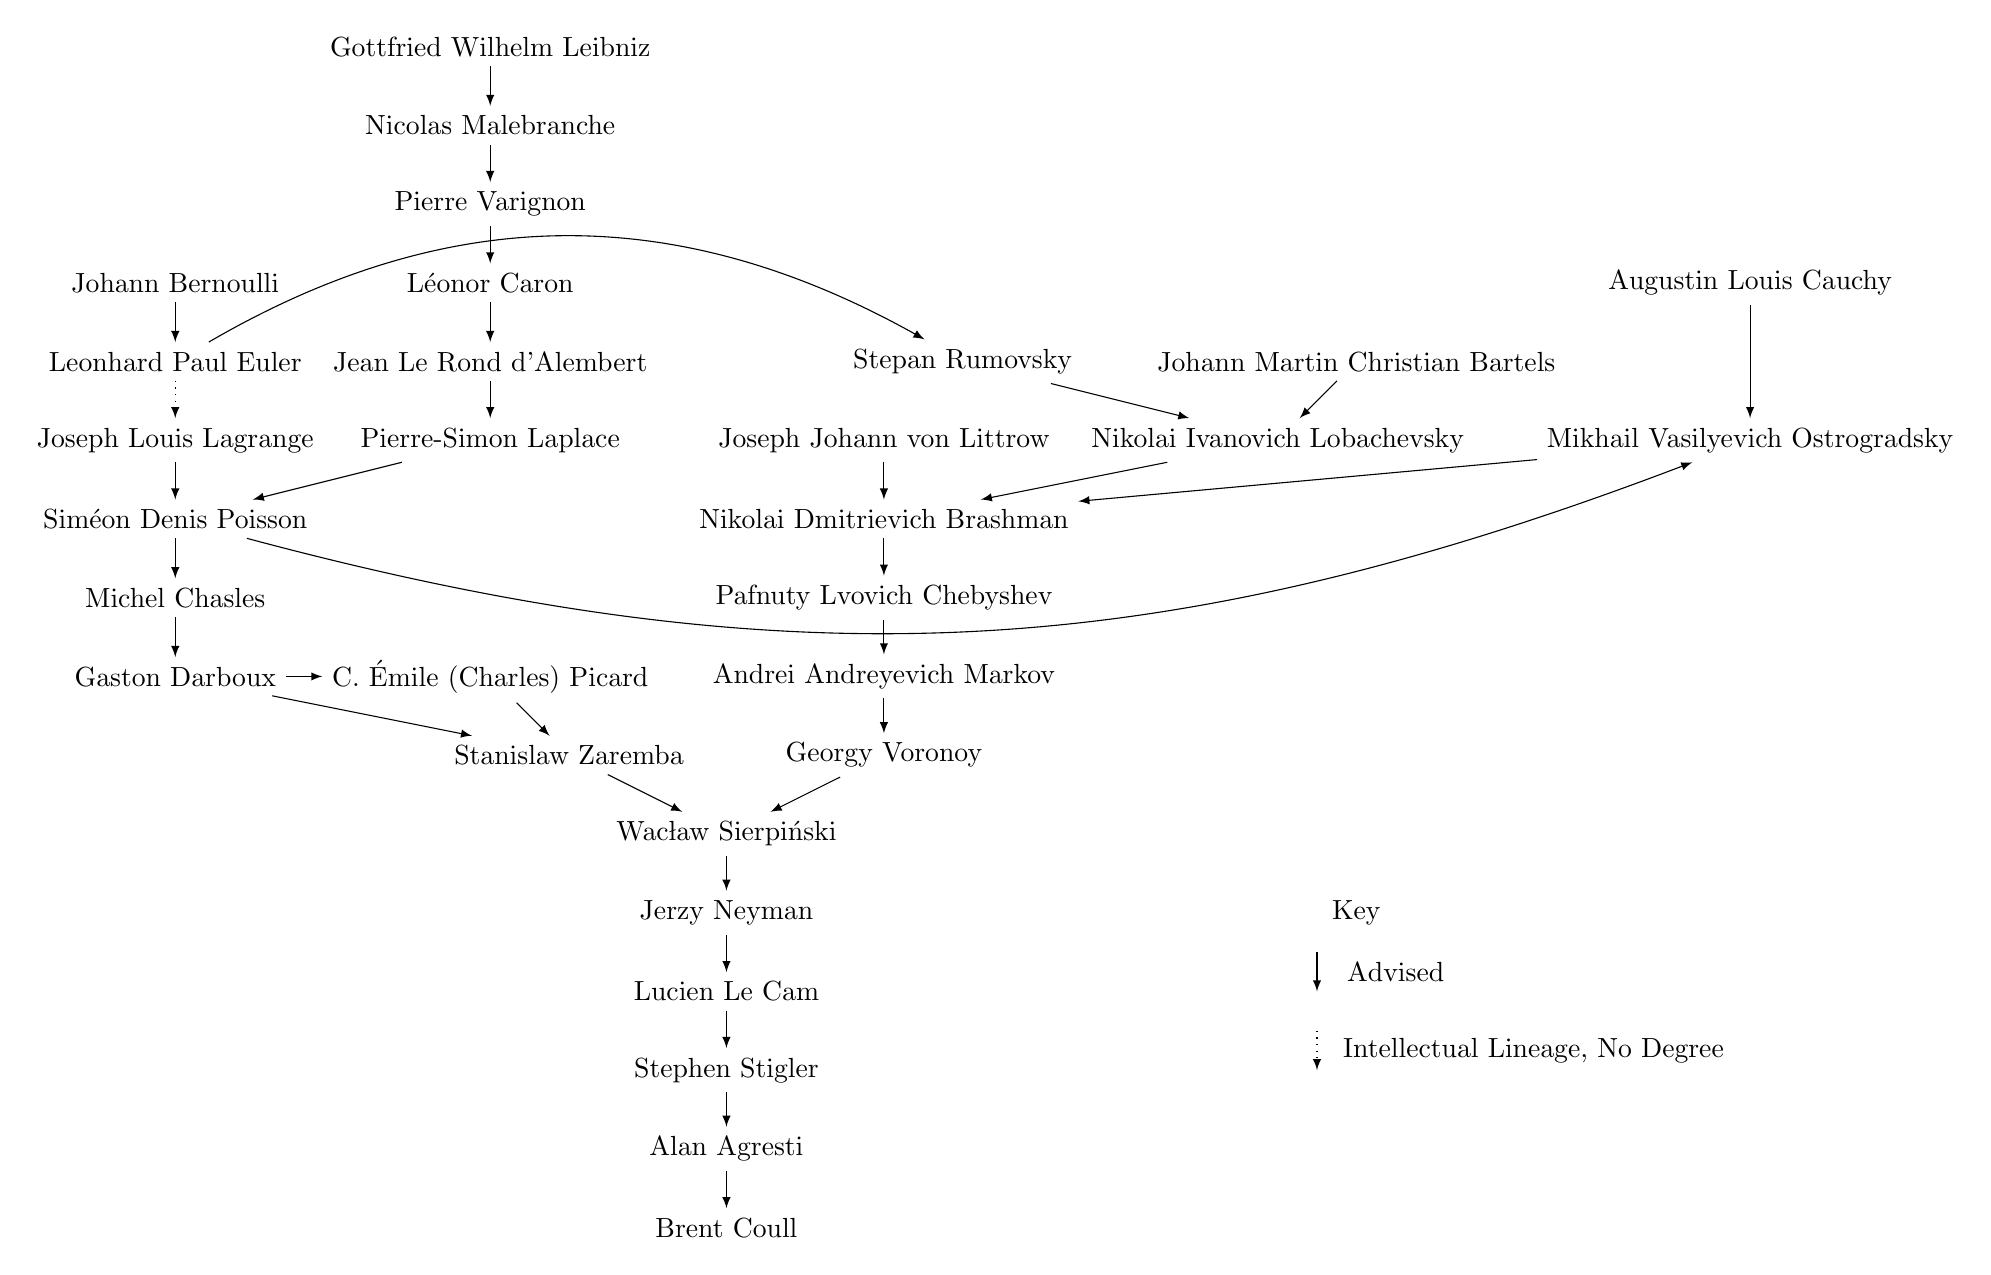
\begin{tikzpicture}

\node (Cauchy) at (13,12) {Augustin Louis Cauchy};
\node (Rumovsky) at (3,11) {Stepan Rumovsky};
\node (Bartels) at (8,11) {Johann Martin Christian Bartels};
\node (Ostrogradsky) at (13,10) {Mikhail Vasilyevich Ostrogradsky};
\node (Lobachevsky) at (7,10) {Nikolai Ivanovich Lobachevsky};
\node (Littrow) at (2,10) {Joseph Johann von Littrow};
\node (Brashman) at (2,9) {Nikolai Dmitrievich Brashman};
\node (Chebyshev) at (2,8) {Pafnuty Lvovich Chebyshev};
\node (Markov) at (2,7) {Andrei Andreyevich Markov};

\node (Leibniz) at (-3,15) {Gottfried Wilhelm Leibniz};
\node (Malebranche) at (-3,14) {Nicolas Malebranche};
\node (Varignon) at (-3,13) {Pierre Varignon};
\node (Caron) at (-3,12) {L\'eonor Caron};
\node (dAlembert) at (-3,11) {Jean Le Rond d'Alembert};
\node (Bernoulli) at (-7,12) {Johann Bernoulli};
\node (Euler) at (-7,11) {Leonhard Paul Euler};
\node (Laplace) at (-3,10) {Pierre-Simon Laplace};
\node (Lagrange) at (-7,10) {Joseph Louis Lagrange};
\node (Poisson) at (-7,9) {Sim\'eon Denis Poisson};
\node (Chasles) at (-7,8) {Michel Chasles};
\node (Picard) at (-3,7) {C. \'Emile (Charles) Picard};
\node (Darboux) at (-7,7) {Gaston Darboux};
\node (Voronoy) at (2,6) {Georgy Voronoy};
\node (Zaremba) at (-2,6) {Stanislaw Zaremba};
\node (Serpinski) at (0,5) {Wac\l{}aw Sierpi\'nski};
\node (Neyman) at (0,4) {Jerzy Neyman};
\node (LeCam) at (0,3) {Lucien Le Cam};
\node (Stigler) at (0,2) {Stephen Stigler};
\node (Agresti) at (0,1) {Alan Agresti};
\node (Coull) at (0,0) {Brent Coull};

\draw [-latex] (Agresti) -> (Coull);
\draw [-latex] (Stigler) -> (Agresti);
\draw [-latex] (LeCam) -> (Stigler);
\draw [-latex] (Neyman) -> (LeCam);
\draw [-latex] (Serpinski) -> (Neyman);
\draw [-latex] (Zaremba) -> (Serpinski);
\draw [-latex] (Voronoy) -> (Serpinski);
\draw [-latex] (Picard) -> (Zaremba);
\draw [-latex] (Darboux) -> (Zaremba);
\draw [-latex] (Darboux) -> (Picard);
\draw [-latex] (Chasles) -> (Darboux);
\draw [-latex] (Poisson) -> (Chasles);
\draw [-latex] (Lagrange) -> (Poisson);
\draw [-latex] (Laplace) -> (Poisson);
\draw [-latex, dotted] (Euler) -> (Lagrange);
\draw [-latex] (Bernoulli) -> (Euler);
\draw [-latex] (dAlembert) -> (Laplace);
\draw [-latex] (Caron) -> (dAlembert);
\draw [-latex] (Varignon) -> (Caron);
\draw [-latex] (Malebranche) -> (Varignon);
\draw [-latex] (Leibniz) -> (Malebranche);

\draw [-latex] (Markov) -> (Voronoy);
\draw [-latex] (Chebyshev) -> (Markov);
\draw [-latex] (Brashman) -> (Chebyshev);
\draw [-latex] (Littrow) -> (Brashman);
\draw [-latex] (Lobachevsky) -> (Brashman);
\draw [-latex] (Ostrogradsky) -> (Brashman);
\draw [-latex] (Bartels) -> (Lobachevsky);
\draw [-latex] (Rumovsky) -> (Lobachevsky);
\draw [-latex] (Euler) to [bend left] (Rumovsky);
\draw [-latex] (Cauchy) -> (Ostrogradsky);
\draw [-latex] (Poisson) to [bend right=18] (Ostrogradsky);

\node at (8, 4) {Key};
\draw [-latex] (7.5, 3.5) to (7.5,3);
\node at (8.5, 3.25) {Advised};
\draw [-latex, dotted] (7.5, 2.5) to (7.5,2);
\node [align=left] at (10.25, 2.25) {Intellectual Lineage, No Degree};

\end{tikzpicture}
\end{document}
